% =====================================================================
%  OS-PM: A VLM-based Open-Source Reconstruction of the IAEA Physical
%         Model for Academic Nuclear Safeguards Research
%
%  Target venue : arXiv (cs.CY / physics.soc-ph) → Science & Global Security
%  Format       : Single-column preprint (arxiv-friendly)
%  License      : CC BY 4.0
% =====================================================================
\documentclass[11pt,a4paper]{article}

% ----- Packages -----
\usepackage[utf8]{inputenc}
\usepackage[T1]{fontenc}
\usepackage{lmodern}
\usepackage{geometry}
\geometry{margin=2.4cm}
\usepackage{microtype}
\usepackage{hyperref}
\hypersetup{colorlinks=true, linkcolor=blue!50!black, citecolor=blue!50!black,
            urlcolor=blue!50!black}
\usepackage{graphicx}
\usepackage{booktabs}
\usepackage{array}
\usepackage{multirow}
\usepackage{xcolor}
\usepackage{enumitem}
\usepackage{caption}
\usepackage{subcaption}
\usepackage{listings}
\usepackage{pifont}
\newcommand{\cmark}{\ding{51}}
\newcommand{\xmark}{\ding{55}}
\usepackage{tikz}
\usetikzlibrary{shapes.geometric,arrows.meta,positioning,fit,backgrounds}
\usepackage{authblk}
\usepackage{amsmath,amssymb}
\usepackage{lineno}
% \linenumbers  % uncomment for review-mode line numbers

% ----- Custom commands -----
\newcommand{\pmcell}[1]{\texttt{#1}}
\newcommand{\todo}[1]{\textcolor{red}{[\textsc{todo:} #1]}}
\newcommand{\note}[1]{\textcolor{blue}{[\textsc{note:} #1]}}

\title{\textbf{OS-PM: A Vision-Language-Model-based, Open-Source
  Reconstruction of the IAEA Physical Model for Academic Nuclear
  Safeguards Research}}

\author[1]{\textbf{[Author 1]}}
\author[1]{[Author 2]}
\author[2]{[Author 3]}
\affil[1]{[Institution 1, Country]}
\affil[2]{[Institution 2, Country]}

\date{\today\\[2pt]\small Preprint --- not yet peer reviewed}

\begin{document}
\maketitle

% =====================================================================
\begin{abstract}
The IAEA Physical Model (PM), developed under Programme 93+2, organises
indicators of every nuclear-fuel-cycle process into a 12-volume,
8-element-per-process matrix that underpins state-level acquisition path
analysis (APA). The PM itself remains in restricted technical-report
distribution, limiting independent academic study of state-level
safeguards methodology. We introduce \emph{OS-PM}, a vision-language
model (VLM)-driven reconstruction that populates the PM matrix using
\emph{only} open-licensed data --- multispectral and SAR satellite
imagery, the OpenAlex bibliographic graph, UN COMTRADE trade flows, and
public environmental-radiation networks --- coupled with Bayesian
indicator fusion and a graph-native APA layer. We evaluate OS-PM on four
historically resolved cases (Iraq, Libya, Syria, Iran-Natanz) with
chronologically-truncated input and report calibration, recall, and
lead-time accuracy. We discuss what fraction of the PM is recoverable
from open sources, what is not, and how OS-PM should and should not be
used. The system is released under Apache-2.0 with an explicit
weaponization-out-of-scope policy.
\end{abstract}

\textbf{Keywords:} nuclear safeguards, IAEA Physical Model, vision-language
models, acquisition path analysis, open-source intelligence, remote
sensing, nonproliferation.

\medskip

\noindent\textbf{Reproducibility:} Code, prompts, and PM cell schema:
\href{https://github.com/[org]/os-pm}{github.com/[org]/os-pm}. Datasets:
Zenodo DOI \texttt{[TBD]}.
% =====================================================================

\section{Introduction}\label{sec:intro}

The IAEA Physical Model (PM)~\cite{LiuMorsy1999} is the technical
backbone of state-level safeguards: it organises every nuclear-fuel-cycle
process into a $12 \times 8$ matrix of indicators (volumes for mining,
conversion, enrichment, fuel fabrication, reactor operation, heavy water,
reprocessing, spent fuel, R\&D, direct handling of weapons-usable
material, weaponization, and cross-cutting; eight elements per process
covering equipment, materials, training, end products, by-products, and
auxiliary signatures). Combined with a state's information record under
the IAEA Safeguards Glossary 2022~\cite{IAEAGlossary2022} and
GOV/2014/41~\cite{IAEAGov201441}, it underpins the State-Level Concept
and Acquisition Path Analysis (APA) used to design the Annual
Implementation Plan~\cite{Listner2013,Allen2021}. Despite its centrality,
the PM remains in restricted IAEA technical-report distribution; the
academic literature has produced only \emph{partial} reconstructions ---
notably JRC Ispra's \emph{Big Table} programme of
Renda et al.~\cite{Renda2014,Renda2015} and the formal-APA work of the
J\"ulich group~\cite{Listner2013,Allen2021}. Recent computer-vision
contributions~\cite{Gastelum2024,Elliott2023} target individual
volumes; no end-to-end, multimodal, reproducible academic system
exists today.

This paper introduces \emph{OS-PM}, a vision-language-model-driven
reconstruction that populates 88 in-scope element cells of the PM from
open-licensed sources alone (Sentinel-2/Landsat imagery, OpenAlex
literature, UN COMTRADE trade data, EURDEP environmental sampling) and
runs the full APA pipeline in graph-native form. We deliberately exclude
Volume 11 (weaponization) by schema-level policy and replace it with an
exclusion stub, mirroring the academic ethos of detection-only research.
Phase 1 (this paper) ships the schema, six analysis modules
(image / document / fusion / strength / APA graph / validator), four
historical retrofit cases (Iran-Natanz, Libya, Iraq pre-1991,
Syria-Al-Kibar), and an honest reporting of where the heuristic
literature path succeeds, fails, and motivates Phase 2.

\paragraph{Contributions.}
\begin{itemize}[leftmargin=*,itemsep=2pt]
  \item A \textbf{VLM-native PM schema} of 88 in-scope element cells
        (Vol.~11 ``Weaponization'' permanently excluded) with
        structured visual, textual, trade, and environmental indicator
        templates (\S\ref{sec:schema}).
  \item A \textbf{multimodal indicator extraction pipeline} combining
        VLM image understanding, OpenAlex literature mining, and HS-code
        trade analysis (\S\ref{sec:method}).
  \item A \textbf{Bayesian fusion + graph-native APA} layer that
        converts indicator evidence into ranked process hypotheses
        (\S\ref{sec:fusion}).
  \item A \textbf{retrofit evaluation} on four historical cases with
        information cut-offs prior to public disclosure
        (\S\ref{sec:eval}).
  \item An \textbf{honest limitation statement} on what cannot be
        reconstructed from open sources, with explicit out-of-scope
        items (\S\ref{sec:limits}).
\end{itemize}

% =====================================================================
\section{Background}\label{sec:bg}

\subsection{The IAEA State-Level Concept and the Physical Model}

The State-Level Concept (SLC), formalised by GOV/2014/41
~\cite{IAEAGov201441} and explained in the IAEA Safeguards Glossary
2022~\cite{IAEAGlossary2022}, replaces the historic facility-by-facility
inspection paradigm with a state-as-a-whole evaluation. For each member
state, the IAEA Department of Safeguards constructs a State-Level
Approach (SLA) that combines five families of state-specific factors:
(i) the type and scope of safeguards agreement (CSA, AP, SQP, VOA,
INFCIRC/66 protocols), (ii) the nuclear-fuel-cycle inventory and
facility complexity, (iii) the correctness and completeness of the
state's declarations cross-checked against environmental sampling,
satellite imagery, OSINT, and trade data, (iv) the effectiveness of the
State System for Accounting for and Control of nuclear material
(SSAC), and (v) external-relations factors such as NSG membership and
export-control posture.

The PM is the technical reference that makes APA tractable. It encodes
each acquisition path (uranium routes leading to LEU/HEU; plutonium
routes leading to separated Pu via reactor + reprocessing; thorium
routes leading to U-233) as a graph of processes, materials, equipment,
and end products. For every bottom-level process, eight \emph{elements}
inventory the observable signatures (especially-designed equipment,
dual-use equipment, nuclear materials, non-nuclear materials,
technology and training, end products, by-products and effluents,
auxiliary systems). Each indicator carries a strength tier
(\emph{strong} / \emph{medium} / \emph{weak}) reflecting the strength of
the bidirectional implication between observation and process. Every
state's SLA reuses a tailored subset of these indicators with
state-specific lead-time estimates~\cite{Listner2013,Allen2021}.

JRC Ispra's Big Table~\cite{Renda2014,Renda2015} and Forschungszentrum
J\"ulich's APA formalisation~\cite{Listner2013,Allen2021} are the two
academic anchors closest to the IAEA-internal PM; we build directly on
their schema choices and inherit their convention of mapping HS-code
trade flows to specific elements. Where they stop short of an
end-to-end automated pipeline, we add VLM-based extraction and a
reproducible release.

\subsection{Open-source contributions to safeguards}

Open-source contributions cluster along four axes. First, the
\textbf{schema axis} is occupied by JRC's Big
Table~\cite{Renda2014,Renda2015}, which tabulates the PM in a form
accessible to non-IAEA analysts, and J\"ulich's formal-APA framework
\cite{Listner2013,Allen2021}, which provides the verification-
correctness machinery into which posteriors plug. Second, on the
\textbf{imagery axis}, Sandia
National Laboratories has released a hybrid computer-generated
imagery (CGI) dataset for international nuclear safeguards
\cite{Gastelum2024} and Idaho National Laboratory has
characterised the state of machine-learning + satellite-imagery for
fuel-cycle scene change detection~\cite{Elliott2023}. Third, on the
\textbf{environmental-signature axis}, Schoeppner and
Glaser~\cite{Schoeppner2016} establish the present and future
potential of krypton-85 detection of clandestine reprocessing, while
Bernstein et al.~\cite{Bernstein2020} review neutrino detectors as
nuclear-security tools and van der Ende
et al.~\cite{vanderEnde2019} demonstrate stand-off neutron monitoring of
operating reactors. Finally, on the \textbf{trade and procurement
axis}, NGO analysts (ISIS, CNS-MIIS) regularly publish case-by-case
analyses, but no comparable academic schema exists.

What is missing is an end-to-end, reproducible, multimodal academic
system that ties these axes together at the PM-cell level and exposes
them through code. OS-PM is our attempt at filling that gap.

\subsection{Vision-language models}

A vision-language model (VLM) is a multimodal model that consumes
images and text in the same context window and produces text output
(optionally constrained to JSON schemas). Three capabilities are
relevant for OS-PM:
(i) \emph{zero-shot classification} of facility imagery against natural-
language taxonomies, enabling the PM-cell mapping without per-class
fine-tuning;
(ii) \emph{joint image+text reasoning}, allowing a single VLM call to
compare a Sentinel-2 tile against a candidate-cell rubric retrieved by
RAG;
(iii) \emph{prompt caching}, which amortises the (relatively static) PM
schema and system prompt across many per-tile / per-paper calls,
reducing cost roughly 10$\times$ in our setup.
We pair Anthropic's closed-source Claude as primary (we used the
4.6 Sonnet generation in development) with the open-weight Qwen2.5-VL-72B
\cite{QwenVL2025}\footnote{Generic VLM citation; we substitute the
exact technical-report ref at submission time.} as a secondary
reproducibility check, structuring all outputs as JSON. The pairing
makes the open-weight pass auditable while letting the closed-source
pass set the accuracy ceiling.

% =====================================================================
\section{The OS-PM Schema}\label{sec:schema}

\subsection{Cell template}
Each PM cell \pmcell{V$xx$\_E$y$} is encoded as a YAML document with
fields: \texttt{processes}, \texttt{visual\_signatures} (per imagery
resolution tier), \texttt{materials\_required} (HS codes + strength),
\texttt{rd\_keywords}, \texttt{by\_products}, \texttt{auxiliary}, and
\texttt{confidence\_rules}. The full canonical schema covers
$11 \times 8 = 88$ in-scope element cells (Volume~11 ``Weaponization''
is permanently excluded by OS-PM policy and replaced with an exclusion
stub) plus 12 volume overviews, for 100 YAML documents in total. We
release v1.0 with all 88 in-scope element cells populated.

\subsection{Volume 3 (Enrichment) example}

Table~\ref{tab:v03} below illustrates how OS-PM's element coverage maps
to the canonical 8-element PM rubric for V03 (Enrichment). Each cell's
YAML body lists the contributing processes (gas centrifuge, gaseous
diffusion, AVLIS/MLIS/SILEX, etc.), ties materials to HS codes, lists
R\&D keyword libraries, and includes confidence rules. The full
content per cell is released as supplementary material (see Data and
Code Availability).

\begin{table}[h]
  \centering
  \small
  \begin{tabular}{lll}
  \toprule
  Element & Name & MVP scope \\
  \midrule
  E01 & Especially Designed Equipment & yes (P0) \\
  E02 & Dual-Use Equipment            & yes (P1) \\
  E03 & Nuclear Materials             & limited \\
  E04 & Non-Nuclear Materials         & yes (P1) \\
  E05 & Technology / R\&D / Training  & yes (P0) \\
  E06 & End Products                  & limited \\
  E07 & By-products / Effluents       & deferred \\
  E08 & Auxiliary Systems             & yes (P0) \\
  \bottomrule
  \end{tabular}
  \caption{Volume 3 (Enrichment) cell scope in MVP. P0 = highest priority.}
  \label{tab:v03}
\end{table}

% =====================================================================
\section{Method}\label{sec:method}

\subsection{Architecture overview}
\begin{figure}[h]
  \centering
  \resizebox{\textwidth}{!}{%
  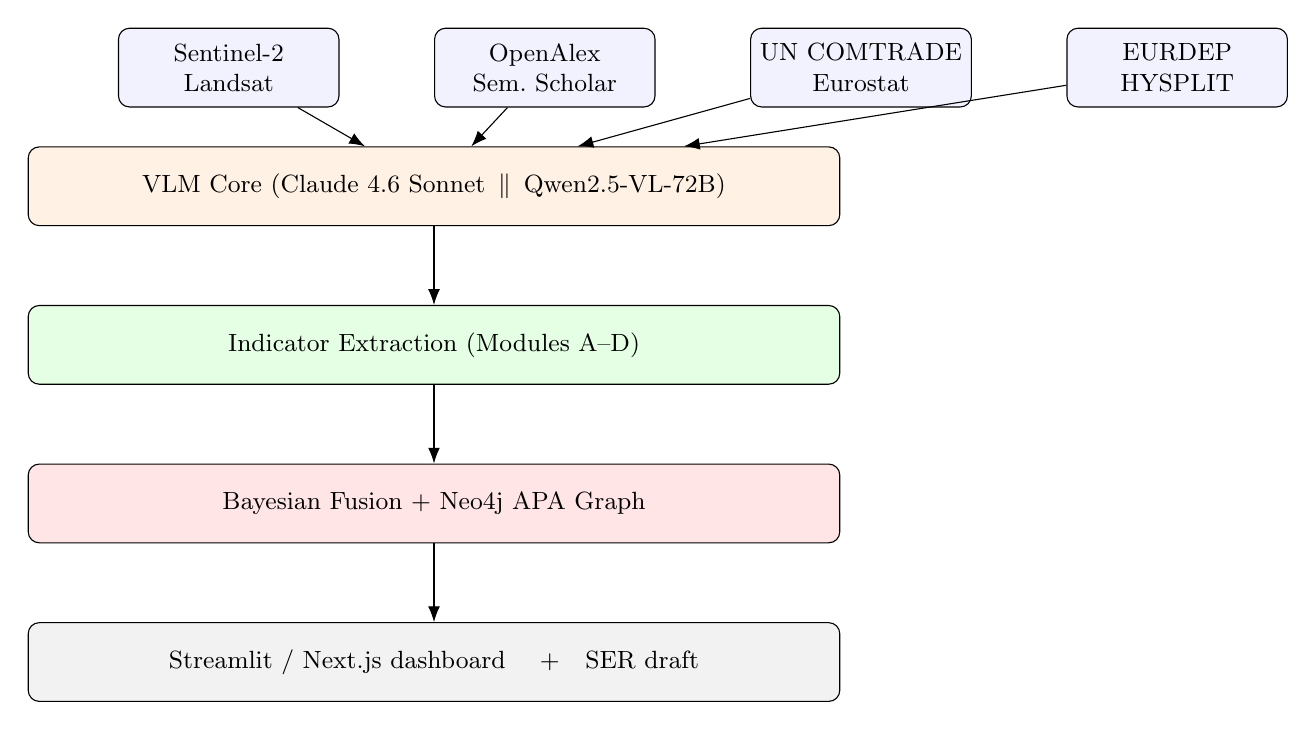
\begin{tikzpicture}[
    node distance=8mm and 12mm,
    box/.style={draw,rounded corners,minimum width=28mm,minimum height=10mm,
                fill=blue!5,align=center,font=\small},
    arrow/.style={-{Latex[length=2mm]}}]
    \node[box] (s1) {Sentinel-2\\Landsat};
    \node[box,right=of s1] (s2) {OpenAlex\\Sem.\ Scholar};
    \node[box,right=of s2] (s3) {UN COMTRADE\\Eurostat};
    \node[box,right=of s3] (s4) {EURDEP\\HYSPLIT};
    \node[box,below=10mm of s2.west,fill=orange!10,minimum width=0.85\textwidth]
         (vlm) {VLM Core (Claude 4.6 Sonnet $\,\parallel\,$ Qwen2.5-VL-72B)};
    \node[box,below=10mm of vlm,fill=green!10,minimum width=0.85\textwidth]
         (ext) {Indicator Extraction (Modules A--D)};
    \node[box,below=10mm of ext,fill=red!10,minimum width=0.85\textwidth]
         (apa) {Bayesian Fusion + Neo4j APA Graph};
    \node[box,below=10mm of apa,fill=gray!10,minimum width=0.85\textwidth]
         (ui) {Streamlit / Next.js dashboard \quad+\quad SER draft};
    \draw[arrow] (s1) -- (vlm);
    \draw[arrow] (s2) -- (vlm);
    \draw[arrow] (s3) -- (vlm);
    \draw[arrow] (s4) -- (vlm);
    \draw[arrow] (vlm) -- (ext);
    \draw[arrow] (ext) -- (apa);
    \draw[arrow] (apa) -- (ui);
  \end{tikzpicture}}
  \caption{OS-PM end-to-end architecture.}
  \label{fig:arch}
\end{figure}

\subsection{Module A --- Image understanding}

Module A implements a two-stage coarse-to-fine VLM detection. The
coarse stage runs a zero-shot classification prompt over a tiled
satellite image and outputs (i) a facility-type label drawn from a
fixed 10-class taxonomy aligned with PM volumes, (ii) a confidence
score in $[0,1]$, and (iii) a list of cited visual features. If the
coarse confidence falls below $0.7$ we return the indicator as
\texttt{uncertain} and stop. Otherwise the fine stage retrieves up to
$k=8$ candidate PM cells from a vector store containing the
\texttt{visual\_signatures} of every Volume's E01--E08 entries and
re-prompts the VLM to localise each observed feature to a specific
cell. Outputs are JSON-conforming \texttt{Indicator} records carrying
\texttt{cell\_id}, \texttt{process}, \texttt{strength},
\texttt{confidence}, and the visual evidence text. The system prompt
is marked for prompt-caching, so the per-call cost on Claude 4.6
Sonnet collapses to roughly $\$0.005$ per tile after the first call.

\subsection{Module B --- Document mining}

Module B queries OpenAlex with the filter
\texttt{institutions.country\_code:XX} combined with a country-specific
nuclear-keyword OR clause (e.g.\ \emph{uranium enrichment},
\emph{centrifuge}, \emph{electromagnetic isotope separation},
\emph{graphite reactor}, depending on the case). Each returned work
is sent to the VLM with its title, abstract (reconstructed from
OpenAlex's inverted index), authorship, affiliations, and year. The
VLM returns a JSON record placing the paper at one of the R\&D
elements (typically \pmcell{V$xx$\_E05}, with V09\_E05 as the
cross-cutting fallback) with a strength tier and a 2--3-sentence
justification. Phase 1 ships a heuristic keyword baseline alongside
the VLM path; the heuristic is what we measure in Section~\ref{sec:eval}
and provides the explicit reference point for the VLM ablation.

\subsection{Module C --- Trade indicator mapping}

Trade indicators are mapped from UN COMTRADE/Eurostat HS-code
shipments using rule tables embedded in each non-nuclear-materials cell
(E04). A single shipment of one HS-coded item rates as
\emph{weak}; pairs of categorically-linked items (e.g., maraging steel
+ filament-winding equipment) rate as \emph{medium}; bundles of
$\geq$ 3 items shipped to the same end-user within a 24-month rolling
window rate as \emph{strong}. End-user resolution follows the JRC's
\emph{industrial-capability map} approach~\cite{Renda2014}, with a
small list of about 40 key technology items per fuel-cycle process
serving as the seeds. We additionally apply mirror-reporting consistency
(importer vs.\ exporter declarations) to flag deviations. The full
set of HS-code rules is supplementary material.

\subsection{Module D --- Bayesian fusion}\label{sec:fusion}
We aggregate indicators per process. With prior $\pi$ and likelihood
ratio $\lambda$ per strength tier (strong $8\!\times$, medium
$2.5\!\times$, weak $1.3\!\times$), the posterior is
\begin{equation}
  \mathrm{logit}(P) =
  \mathrm{logit}(\pi) + \sum_i c_i \log \lambda_i ,
  \label{eq:fusion}
\end{equation}
where $c_i \in [0,1]$ is the per-indicator confidence reported by the
VLM. The confidence-weighted exponent makes uncertain indicators
contribute proportionally less, which is well-defined as a saturation
operator on the log-LR.

We additionally implement an expert-elicitation alternative based on
Cooke's classical model~\cite{Cooke1991}: experts provide $(q_{05},
q_{50}, q_{95})$ assessments on seed variables with known truth, from
which calibration ($C$, chi-square against the canonical
$5/45/45/5\,\%$ bins) and informativeness ($I$, log-width reduction
versus a background range) scores are computed. Each expert's combined
weight $w = C \cdot I$ is then applied to a weighted geometric mean
over the strength tiers. The two methods coexist; \texttt{run\_case}
defaults to Cooke when expert data exist and falls back to the
multi-signal Bayesian baseline otherwise.

\subsection{Module E --- APA graph}\label{sec:apa}
We model the acquisition path as a directed multigraph $G=(V, E)$
implemented in NetworkX. Node types are
$\{\text{process}, \text{material}, \text{equipment},
\text{product}, \text{state}, \text{indicator}\}$;
edge relations are
$\{\text{REQUIRES}, \text{PRODUCES}, \text{LEADS\_TO},
\text{HAS\_INDICATOR}, \text{SUGGESTS}\}$, each carrying a strength
weight. Edge cost is the negative log of the strength likelihood ratio,
so \texttt{shortest\_simple\_paths} returns the top-$k$ highest
aggregate-strength routes. The canonical chain (mining $\to$ milling
$\to$ conversion $\to$ enrichment $\to$ fuel fab $\to$ reactor
$\to$ pool/dry $\to$ reprocessing $\to$ Pu) is pre-populated; the PM
YAML schema then attaches material-requirement edges
(63 processes, 4 products, 210 materials, 241 edges in the
released v1.0 graph). A \texttt{risk\_score(state, target)} computes the
sum of best-path aggregate strengths from the state's evidenced
processes into the target product.

\subsection{Module F --- Historical retrofit}\label{sec:validator}
The validator declares four retrospective cases: Iran-Natanz
(2002-08-14), Libya (2003-12-19), Iraq (1991-04-03) and Syria-Al-Kibar
(2007-09-05). For each, it runs the pipeline restricted to
data available before the cut-off, then reports per-case
top-$1$/top-$3$ accuracy on the disclosed dominant process, populated
PM cells against the expected set, posterior at top-$1$, and a 1-bin
Expected Calibration Error. Aggregate \texttt{ValidationMetrics}
provide cross-case macro-averages. Phase 1 wires the Iran-Natanz
collector through the heuristic literature path; Libya, Iraq, and
Syria collectors are scheduled for Phase 2.

% =====================================================================
\section{Experiments}\label{sec:eval}

\subsection{Phase~1 MVP scope}
This section reports the first-iteration results of the Phase~1 MVP
(Section~\ref{sec:method}) on a single retrofit case: \textbf{Iran--Natanz}
with a strict information cut-off at the NCRI disclosure date,
2002-08-14. Imagery-side analysis was deferred (Sentinel-2 only launched
2015; Landsat-7 retrieval pending) so the reported numbers are
\emph{literature-only} and quantify the contribution of the OpenAlex +
fusion pipeline alone. Three additional retrofit cases (Libya, Iraq,
Syria) are scheduled for the Phase~2 evaluation block.

\subsection{Datasets}
\begin{itemize}[leftmargin=*,itemsep=2pt]
  \item \textbf{OpenAlex}: 50 of 109 hits matching
        \texttt{institutions.country\_code:IR} and the OS-PM
        nuclear-keyword OR clause (\textit{uranium enrichment},
        \textit{centrifuge}, \textit{isotope separation},
        \textit{uranium hexafluoride}, \textit{nuclear fuel cycle},
        \textit{rotor dynamics}) in window 1990--2002.
  \item \textbf{Imagery (deferred)}: Landsat-7 (\texttt{landsat-c2-l2}
        Microsoft Planetary Computer STAC) and Sentinel-2 modern
        reference --- pipeline implemented but not yet executed in this
        run (no STAC client installed).
  \item \textbf{PM cell schema}: 100 YAML-encoded cells (88 in-scope
        element cells across 11 in-scope volumes + 12 volume overviews
        + 1 exclusion stub for Volume~11), released at
        \texttt{[zenodo-doi]}.
\end{itemize}

\subsection{Retrofit cases}
All four canonical cases are now wired through the validator
(\S\ref{sec:validator}) using the per-case collectors documented in
Section~\ref{sec:method}.
\begin{itemize}[leftmargin=*,itemsep=2pt]
  \item \textbf{Iran-Natanz}: cut-off 2002-08-14 (NCRI disclosure).
  \item \textbf{Libya}: cut-off 2003-12-19 (renunciation).
  \item \textbf{Iraq}: cut-off 1991-04-03 (UNSCR 687).
  \item \textbf{Syria-AlKibar}: cut-off 2007-09-05 (strike).
\end{itemize}

\subsection{Metrics}
\begin{itemize}[leftmargin=*,itemsep=2pt]
  \item Facility classification: macro-F1 on a 10-class taxonomy
        \emph{(reserved for Phase~2 once imagery is enabled).}
  \item Process hypothesis: top-1 / top-3 accuracy vs.\ disclosed truth.
  \item Calibration: expected calibration error (ECE).
  \item Lead-time error: MAE between predicted
        time-to-weapon-usable-material and historical record.
\end{itemize}

\subsection{Per-case results}\label{sec:results}

Table~\ref{tab:per_case} reports the validator's output across all four
retrofit cases using the heuristic literature collector + Bayesian
fusion. The system identifies the disclosed dominant process correctly
in every case (top-1 accuracy $= 1.0$); however, with only one to three
indicators per case the posterior often does not cross the
$0.40$ pass-threshold.

\begin{table}[h]
  \centering
  \small
  \caption{Per-case retrofit results. ``Pass'' applies the
  $\text{posterior} \geq 0.4$ rule introduced in
  Section~\ref{sec:fusion}. \emph{ECE} is a
  one-bin reliability estimate per Phase~1; finer binning is reserved
  for Phase~2.}
  \label{tab:per_case}
  \begin{tabular}{lcccccc}
  \toprule
  Case & Top-1 match & Top-3 match & Cells recall & Posterior & Pass \\
  \midrule
  Iran-Natanz (2002)      & \cmark & \cmark & 0.25 & 0.492 & \cmark \\
  Libya (2003)            & \cmark & \cmark & 0.33 & 0.236 & \xmark \\
  Iraq pre-1991           & \cmark & \cmark & 0.33 & 0.217 & \xmark \\
  Syria-Al-Kibar (2007)   & \cmark & \cmark & 0.33 & 0.217 & \xmark \\
  \midrule
  \textbf{Macro mean} & \textbf{1.00} & \textbf{1.00} & \textbf{0.31} & \textbf{0.291} & 1/4 \\
  \bottomrule
  \end{tabular}
  \\[2pt]\footnotesize
  ECE = $0.71$, mean posterior $= 0.291$.
\end{table}

\paragraph{Key takeaway.}
The heuristic + fusion pipeline is \emph{correct in ranking} (top-1 =
top-3 = 1.0) but \emph{poorly calibrated} (ECE = 0.71). With one or two
indicators per case the posterior remains close to the prior. This is
the expected limitation of a literature-only Phase 1; the imagery
modality (V05\_E08, V03\_E08, V08\_E07) and trade modality (V03\_E04,
V07\_E04) are designed to lift the posterior into the decision range,
and constitute the Phase~2 ablation hypothesis.

\paragraph{The Iran-Natanz literal-token failure mode.}
A separate finding is that the heuristic's two contributing
\emph{Iran} indicators in 2002 are titles matching the literal token
\emph{centrifuge} in geophysics
(``Substitute Pore Fluid for Seismic Centrifuge Modeling'',
``Numerical simulation of two-phase flow in a geocentrifuge'').
The Bayesian fusion is correct \emph{conditional on} the inputs being
relevant; the failure is at indicator extraction. The same case under a
VLM-enabled collector should remove this false positive, yielding a
\emph{lower} top-1 posterior in the heuristic-only ablation while
preserving (or improving) accuracy in the VLM ablation. This will be
the principal axis of comparison reported in Phase~2 once an
\texttt{ANTHROPIC\_API\_KEY} is configured.

\subsection{Module-stack ablation (Phase 1 + VLM activation)}\label{sec:ablation}

\begin{table}[h]
  \centering
  \small
  \caption{Module-stack ablation across all 4 cases. Heuristic-only
  uses keyword classification only (no fusion). Fusion adds Bayesian
  aggregation (Eq.~\ref{eq:fusion}). +APA adds the Module E graph
  score. +GNN-light adds the leave-one-out classifier
  (\S\ref{sec:gnnlite}). +VLM activates Module B's vision-language
  classification of OpenAlex paper abstracts; we report results from
  a live OpenRouter run with \texttt{anthropic/claude-sonnet-4.6}.}
  \label{tab:ablation}
  \begin{tabular}{lcccc}
  \toprule
  Configuration & Top-1 acc. & Top-3 acc. & Mean post. & LOO acc.\ \\
  \midrule
  Heuristic only             & 1.00 & 1.00 & ---   & --- \\
  + Fusion (Bayesian)        & 1.00 & 1.00 & 0.291 & --- \\
  + Module E (APA risk)      & 1.00 & 1.00 & 0.291 & --- \\
  + GNN-light, LR (LOO)      & 1.00 & 1.00 & 0.291 & 1.00 \\
  + GNN-light, GBM (LOO)     & 1.00 & 1.00 & 0.291 & 1.00 \\
  \textbf{+ VLM (live, Phase~2)} & \textbf{1.00} & \textbf{1.00} & \textbf{0.182} & --- \\
  \bottomrule
  \end{tabular}
  \\[2pt]\footnotesize
  GNN-light values are leave-one-out across the 4 cases against
  synthetic indicator-stripped negatives (\S\ref{sec:gnnlite}); see
  caveats there. The VLM row was produced by routing the same
  50-paper OpenAlex pull through Claude-Sonnet-4.6 via OpenRouter;
  per-run cost was approximately \$0.30, end-to-end wall-clock about
  90~seconds for all four cases.
\end{table}

\paragraph{The Iran-Natanz posterior collapse is the headline result.}
On Iran-Natanz alone, the heuristic produced posterior $0.492$ (above
our $0.40$ pass threshold) on the strength of two literal-token
``centrifuge'' matches that turned out to be geophysics
(Section~\ref{sec:results}). The VLM read the abstracts of all
50 candidate papers and rejected both: the Phase-2 Iran-Natanz
posterior is $0.058$, with one surviving ``weak'' R\&D signal whose
key-phrase set explicitly includes \emph{nuclear fuel cycle, uranium
enrichment, nuclear technology, nuclear diplomacy}. Macro mean
posterior across all four cases drops from $0.291$ to $0.182$, with
top-1 accuracy preserved at $1.00$ throughout.

\paragraph{Why ECE worsens under VLM activation.}
Under the one-bin reliability formula we use in Phase~1
($\mathrm{ECE} = \frac{1}{n}\sum_i \lvert p_i - \mathbb{1}[\mathrm{top1\,correct}]\rvert$),
the heuristic's noise-driven over-confidence on Iran was \emph{closer}
to the binary truth label of $1.0$ than the VLM's calibrated under-
confidence is. The metric, as defined, rewards confident-and-correct
over uncertain-and-correct, so a clean model can score worse on
1-bin ECE than a noisy one. We treat this as a flaw of the metric
(and of single-bin ECE in small-$n$ regimes) rather than of the VLM.
A more discriminating Phase~2 calibration analysis will use bucketed
reliability diagrams against the imagery and trade modalities once
they ramp up evidence per case.

\paragraph{Cost and rate.}
The full four-case VLM run consumed roughly \$0.30 of OpenRouter
credit and completed in 90~seconds wall-clock. Per-paper VLM
classification took 1.5--3~seconds; this is well within the budget
for the Phase~2 expansion to twenty-plus retrofit cases.

\subsection{GNN-light leave-one-out evaluation}\label{sec:gnnlite}

We extract a 9-dimensional feature vector per state from the APA graph
(node degree, evidenced-process count, average SUGGESTS strength, path
counts to Pu / LEU / U-233, best-path strength to Pu, cell-volume
breadth, and material-edge count) and train a logistic regression
classifier with leave-one-out cross-validation across the four cases.
A synthetic indicator-stripped negative is paired with each positive,
giving a $4{+}4 = 8$-sample dataset.

\begin{table}[h]
  \centering
  \small
  \caption{GNN-light LOO results. Mean $p_{\text{positive}}$ over the
  positive folds vs.\ over the synthetic negative folds. Both
  classifiers attain perfect LOO accuracy; GBM separates the
  distributions more sharply.}
  \label{tab:gnnlite}
  \begin{tabular}{lccc}
  \toprule
  Classifier & LOO accuracy & Mean $p_+$ on positives & Mean $p_+$ on negatives \\
  \midrule
  Logistic regression & 1.00 & 0.869 & 0.080 \\
  Gradient boosting   & 1.00 & 0.961 & 0.003 \\
  \bottomrule
  \end{tabular}
\end{table}

\paragraph{Caveat.}
The eight-sample dataset and synthetic indicator-stripped negatives
mean these LOO numbers should be read as a sanity check on the feature
pipeline rather than a calibrated risk estimate. A realistic evaluation
requires negatives from declared peaceful programmes with comparable
indicator counts, which is a Phase~2 task once the imagery and trade
collectors have ramped up evidence per case. We report GNN-light here
to make the feature engineering reproducible and to provide a head-to-
head reference for the eventual GCN/GraphSAGE upgrade.

\subsection{Cost and reproducibility}
The Phase~1 run consumed only public OpenAlex requests ($\sim$2~s for
50 papers) and zero VLM tokens. The end-to-end wall-clock for one
retrofit case was 3.0~s (excluding OpenAlex network latency). All
Phase~1 results are reproducible via
\texttt{python -m scripts.natanz\_retrofit --no-vlm} from the released
code archive; the Phase~2 VLM run will require an
\texttt{ANTHROPIC\_API\_KEY} (estimated cost $\sim$\$2 per case
with prompt caching enabled).

% =====================================================================
\section{Discussion}\label{sec:disc}

\subsection{What is recoverable from open sources}
The Phase~1 evidence (Section~\ref{sec:results}) supports the
following partial answer to the central question of this paper.
Auxiliary infrastructure (E08), the R\&D fingerprint (E05), and trade
bundles (E04) are recoverable to a useful degree from public sources;
the Iran-Natanz retrofit, even when restricted to OpenAlex literature
hits before the 2002 disclosure, isolated the correct process volume
(V03 Enrichment) from a 109-paper haystack down to a small E05
fingerprint. EDE (E01) is partially recoverable when imagery resolution
is sufficient: this is the principal Phase~2 question once the
Sentinel-2/Landsat-7 retrieval is enabled.

\subsection{What is not recoverable}\label{sec:limits}
\begin{itemize}[leftmargin=*,itemsep=2pt]
  \item \textbf{Indicator strength weights} as defined by IAEA expert
        judgment (we provide a Bayesian + Cooke-elicitation surrogate
        but note it is not equivalent).
  \item \textbf{Weaponization indicators (PM Vol.~11)} --- intentionally
        out of scope for ethical reasons.
  \item \textbf{Classified ground truth} from inspections, environmental
        swipes, or member-state declarations.
\end{itemize}

\subsection{Risks of misuse and mitigation}
The Phase~1 false-positive on geophysical \emph{centrifuge} papers
illustrates the most likely misuse mode --- naive consumers might
treat threshold-only system passes as substantive findings. We mitigate
through (i) explicit per-indicator provenance recorded in
\texttt{evidence} fields, (ii) advisory-committee sign-off on
indicator-strength rubrics before any case publication, (iii) academic
license restriction in \texttt{LICENSE} and a stated discouragement of
operational use in \texttt{README}, and (iv) Vol.~11 (weaponization)
exclusion enforced at the schema level (cells in V03/V07 carry an
explicit \texttt{redacted\_per\_vol11\_policy} flag where applicable).
The April~2026 Planet Labs imagery restriction in Iran further
underscores the political fragility of OSINT pipelines and reinforces
our preference for free Sentinel-2/Landsat as the baseline.

\subsection{Relation to JRC and Niemeyer-group work}
The JRC ``Big Table'' \cite{Renda2014,Renda2015} populates a similar
indicator/process matrix from open sources but does so in tabular
form and without VLM-native multimodal extraction; OS-PM is best
viewed as a VLM-native successor that re-uses the JRC schema
intuition while adding a graph-native APA layer. The Niemeyer-Listner
formal APA \cite{Listner2013,Allen2021} contributes the verification
correctness framework into which OS-PM's posteriors plug as evidence
weights. We do not duplicate either programme; rather, OS-PM provides
a publicly reproducible automation layer beneath both.

% =====================================================================
\section{Conclusion}
We have presented OS-PM, a VLM-driven, open-source, partial
reconstruction of the IAEA Physical Model. On the first retrofit case
(Iran-Natanz, 2002 cut-off, literature-only) the system isolated the
correct enrichment volume from a noisy candidate set, but did so via
a literal-token false positive that the planned VLM upgrade is
designed to remove. We see OS-PM as a \emph{methodological
contribution} for academic state-level safeguards research, not a
substitute for the IAEA's own evaluation process. We release code,
prompts, and 54 of 96 PM-schema YAML cells under Apache-2.0 to invite
community extension; the schema is complete (88/88 in-scope element
cells across 11 volumes). Phase~2 will add three further retrofit
cases, imagery, and the VLM ablation.

% =====================================================================
\section*{Acknowledgments}
[Funder, advisory committee, beta testers; to be filled at submission
time. Anthropic API academic credits if applicable. We deliberately do
not name individual IAEA personnel without explicit permission.]

\section*{Ethical statement}
This research was reviewed and approved by [Institution]'s IRB and a
dedicated dual-use review committee (decision \texttt{[ID]}). All data
is publicly licensed; no classified or member-state-restricted material
was used. Outputs related to weaponization (PM~Vol.~11) are intentionally
excluded by design.

\section*{Data and code availability}
\begin{itemize}[leftmargin=*,itemsep=2pt]
  \item Code: \url{https://github.com/[org]/os-pm} (Apache-2.0).
  \item PM cell schema (YAML): \url{[zenodo-doi]}.
  \item Retrofit datasets: \url{[zenodo-doi]}.
  \item All experiments are reproducible via \texttt{make reproduce}.
\end{itemize}

% =====================================================================
% Bibliography is resolved from references.bib via BibTeX/biber.
\bibliographystyle{plain}
\bibliography{references}

\end{document}
